\section{Configuraciones iniciales}

\subsection{Estructuras cristalinas}

En este capítulo se estudian las propiedades de las estructuras amorfas Li$_x$Si
para distintos valores de $x$ en un rango que va de 0.21 a 4.2. Para algunas de
estas concentraciones se encuentran estructuras cristalinas, las cuales 
fueron extraídas del Materials Project ~\cite{materials_project} 
(mp-1314, mp-672287, mp-569849, mp-29720) y sus posiciones utilizadas para definir
los estados iniciales. Las celdas primitivas de las estructuras cristalinas se
muestran en la figura \ref{fig:cristalinas}, donde están en orden creciente de 
concentración de Li. Las mismas son Si, LiSi, Li$_{12}$Si$_7$, Li$_7$Si$_3$, 
Li$_{13}$Si$_4$, Li$_{15}$Si$_4$, Li$_{21}$Si$_5$ y Li. En la estructura de LiSi
se tiene una remanencia del diamante de Si en los enlaces, en la Li$_{12}$Si$_7$ 
hay dos tipos de clusters de átomos de Si, pentágonos y estrellas, en la
Li$_7$Si$_3$ los átomos de Si se encuentran en mancuernas, en la Li$_{13}$Si$_4$ 
se tienen las mismas mancuernas junto a algunos átomos aislados y, por último, 
todos los átomos de Si se encuentran aislados tanto en la Li$_{15}$Si$_{4}$ como
en la Li$_{21}$Si$_5$. Estas estructuras cristalinas fueron observadas a 
temperaturas altas ~\cite{wen1981}, pero no se encuentran en el funcionamiento de
una batería ~\cite{obrovac2004}. Sin embargo, sus posiciones pueden tomarse como 
iniciales para simular estructuras amorfas a las concentraciones correspondientes.
\begin{figure}[t]
    \centering
    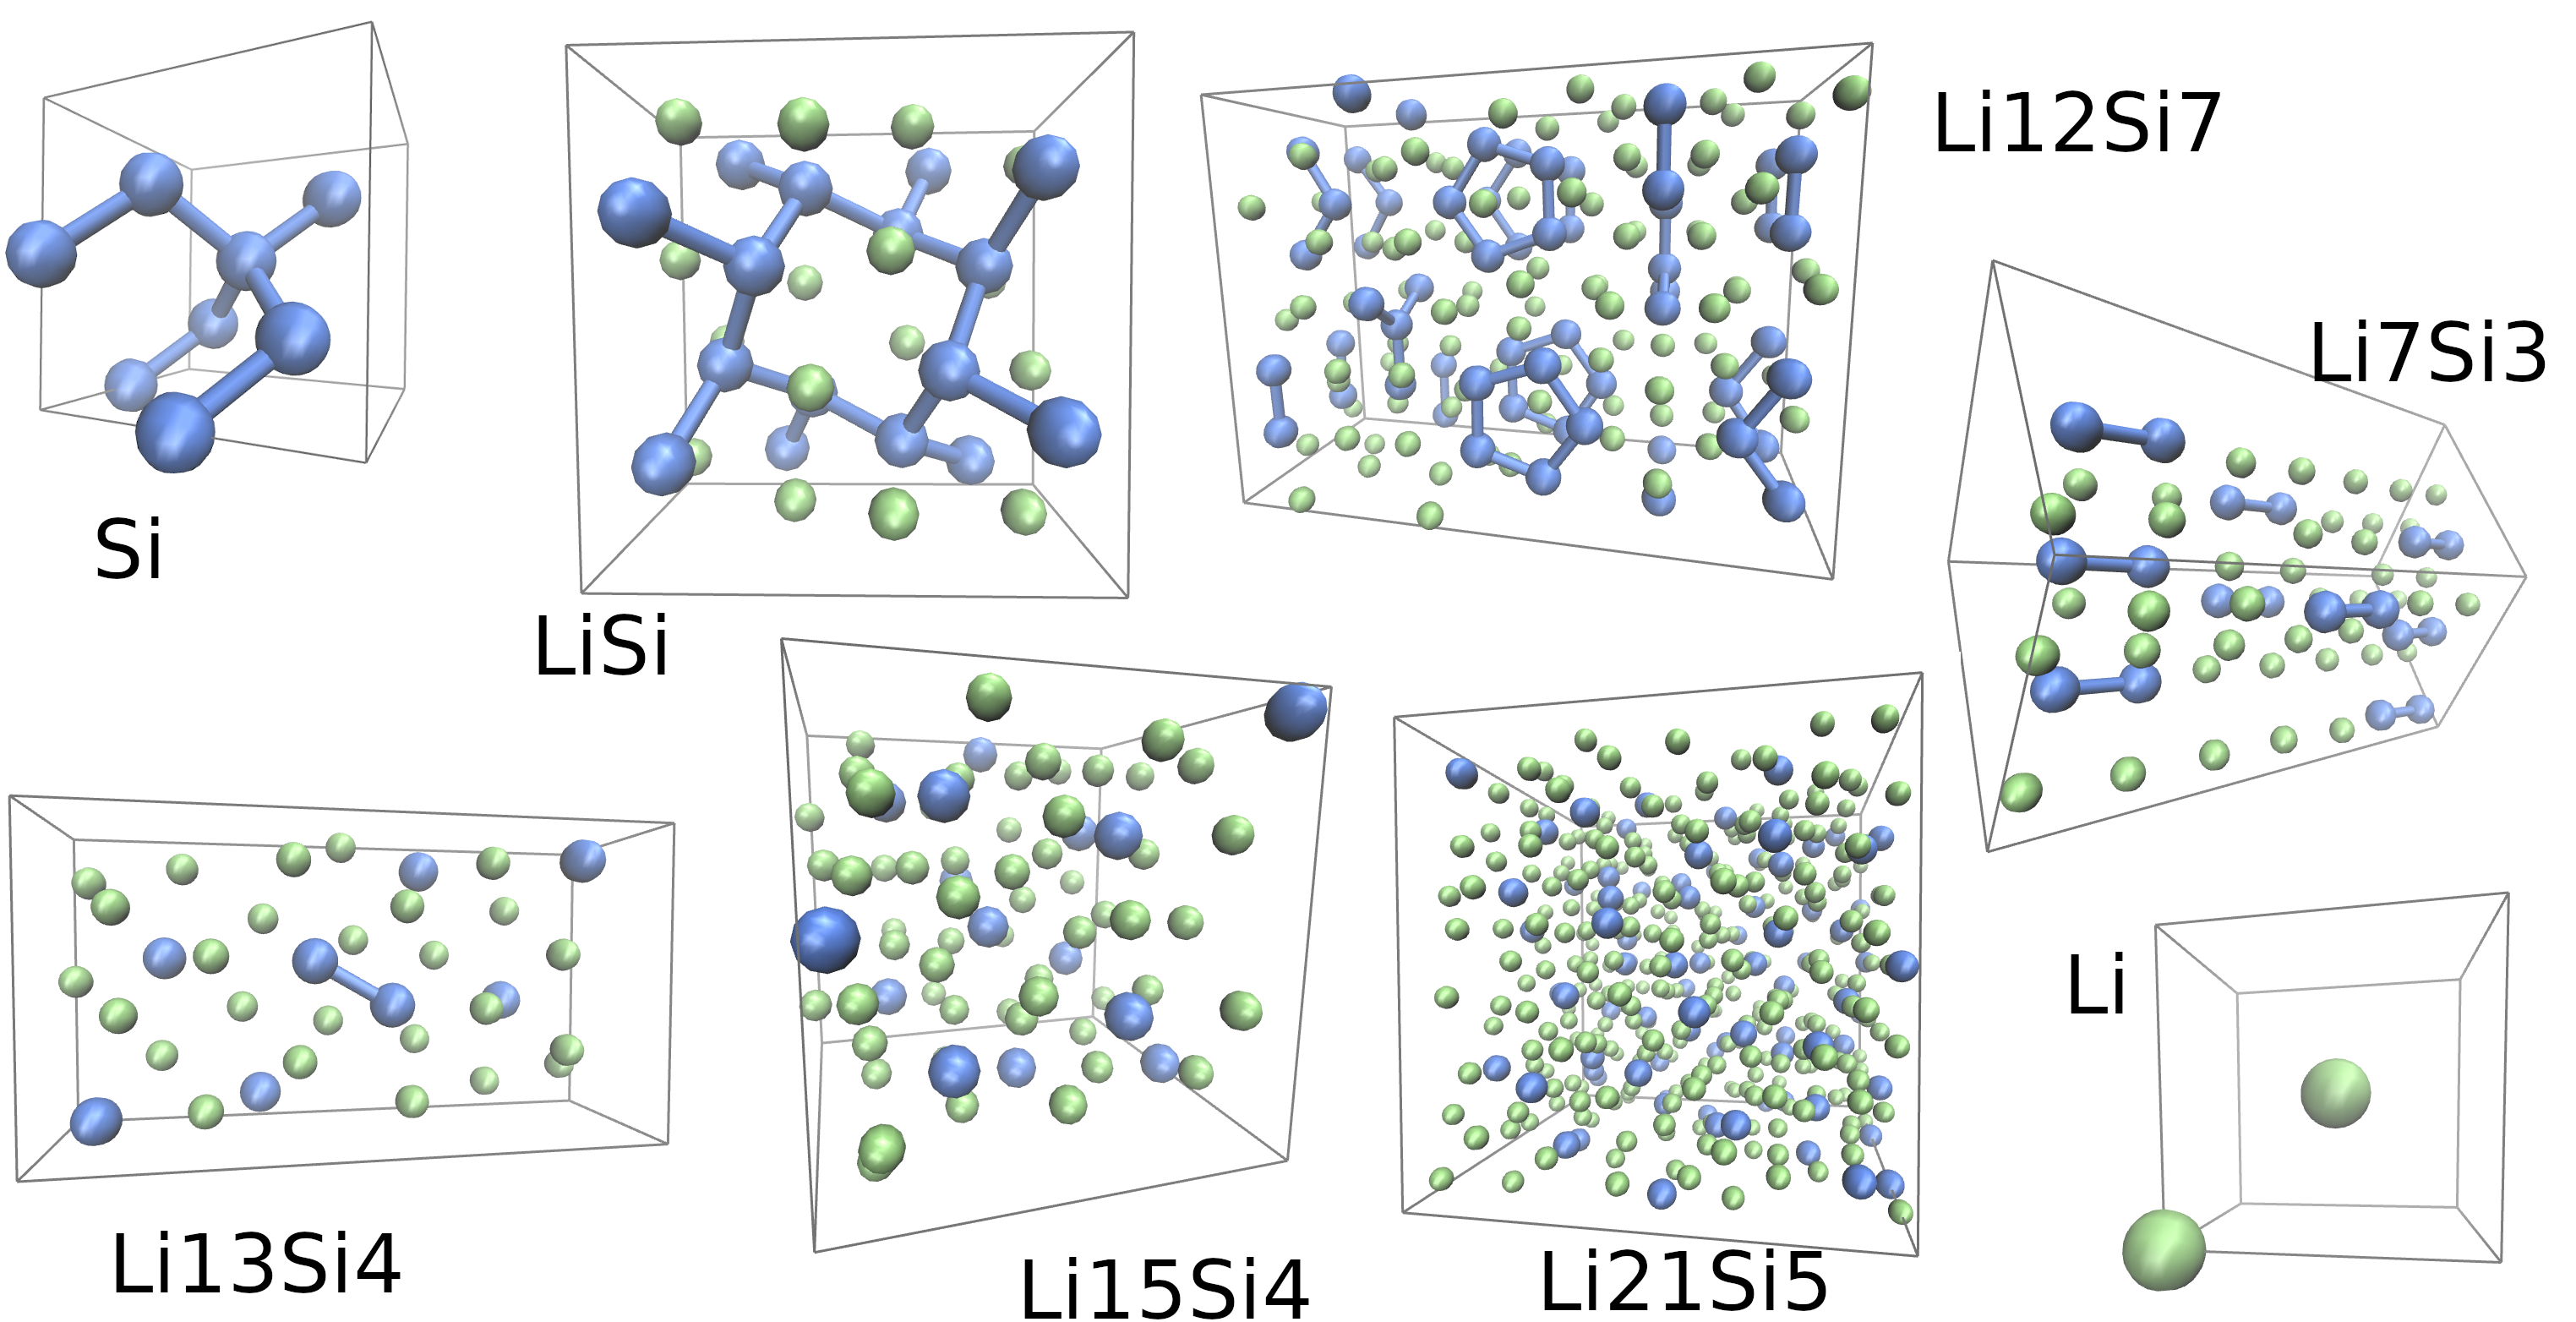
\includegraphics[width=\textwidth]{caracterizacion/config/cristalinas.png}
    \caption{Estructuras cristalinas de Li-Si. Las estructuras no están a escala 
    entre sí. Los átomos de Si se muestran en azul y los de Li en verde, mientras
    que la celda periódica en gris. Los enlaces de Si-Si están graficados si la 
    distancia entre dos de estos átomos es menor a 2.5\AA.}
    \label{fig:cristalinas}
\end{figure}

\subsection{Protocolo de delitiación}

Para obtener configuraciones iniciales para valores de $x$ distintos a los de las 
cristalinas se siguió un protocolo de delitiación, en el cual se selecciona la 
estructura cristalina más cercana con un valor de $x$ superior al deseado,
se le extrae un átomo de Li de manera aleatoria y se realiza una dinámica en el 
ensamble NPT durante 2 ps para relajar el volumen. Para estas simulaciones se 
utilizó el termostato de Nosé-Hoover ~\cite{nose1984a, nose1984b, hoover1985} a
300.0 K, un barostato a 0.0 atm y un paso temporal de 1 fs utilizando el
software \path{LAMMPS} ~\cite{lammps1, lammps2}. La extracción del átomo de Li y
la simulación en el ensamble NPT fueron repetidas hasta alcanzar una concentración
deseada. Por último, para algunas concentraciones en particular, se seleccionó la
estructura con la menor presión absoluta como estado inicial para la exploración 
acelerada de mínimos locales que se introduce en la siguiente sección.
